\documentclass{officialexam} 
\usepackage{circuitikz}
\everymath{\color{blue}}
\definecolor{qqqqff}{rgb}{0,0,1}
\usepackage{graphicx}
\graphicspath{ {./images/} }
\begin{document}
	\maketitle\\
	\borderline{ប្រធាន}
	\begin{enumerate}[I]
		\item (៦ ពិន្ទុ) តើបាតុភូតអូតូអាំងឌុចស្យុងម៉ាញេទិចកើតឡើងនៅពេលណា?
		\item (៦ ពិន្ទុ) ចូររៀបរាបពីវគ្គទាំងបួននៃម៉ាសុីនបន្ទុះបួនវគ្គ។ តើវគ្គណាមួយដែលជាវគ្គបង្កើតកម្មន្តមេកានិច?
		\item (១៥ ពិន្ទុ) នៅភាពដើម $P_i~;~V_i$ និង $T_i$  នៃឧស្ម័នបរិសុទ្ធមួយត្រូវបានឆ្លងកាត់មួយវដ្តនៃដំណើរការដូចបានបង្ហាញក្នុងរូប។
		\begin{multicols}{2}
			\begin{enumerate}[k]
				\item គណនាកម្មន្តសរុបក្នុងមួយវដ្តនៃដំណើរការ។
				\item គណនាបរិមាណកម្តៅសរុបក្នុងមួយវដ្តនៃដំណើរការ។
				\item ចូរអនុវត្តន៍ជាលេខ ដើម្បីគណនាកម្មន្តសរុបក្នុងមួយវដ្តនៃដំណើរការដូចរូប ។ បើ $1.0mol$ នៃឧស្ម័នស្ថិតនៅសីតុណ្ហភាព $0^\circ C$។ \\គេឱ្យ ថេរសកលនៃឧស្ម័ន $R=8.31J/mol\cdot K$
			\end{enumerate}
			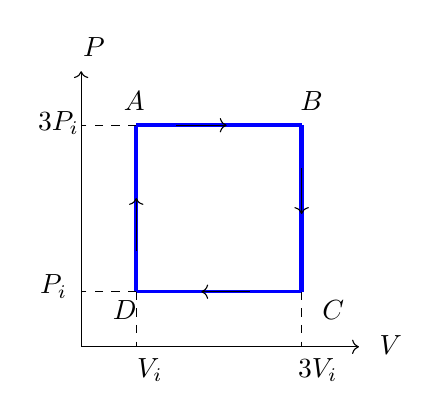
\begin{tikzpicture}[x=1.0cm,y=1.0cm, scale=0.7]
			\draw [->] (-1,0) -- (-1,5);
			\draw [->] (-1,0) -- (4.04,0);
			\draw [line width=1.6pt,color=qqqqff] (0,1)-- (0,4.02);
			\draw [line width=1.6pt,color=qqqqff] (0,4.02)-- (3,4.02);
			\draw [line width=1.6pt,color=qqqqff] (3,4.02)-- (3,1);
			\draw [line width=1.2pt,color=qqqqff] (0,1)-- (3,1);
			\draw [dash pattern=on 3pt off 3pt] (0,1)-- (0,0);
			\draw [dash pattern=on 3pt off 3pt] (3,1)-- (3,0);
			\draw [dash pattern=on 3pt off 3pt] (0,1)-- (-1,1);
			\draw [dash pattern=on 3pt off 3pt] (0,4.02)-- (-1,4.02);
			\draw (-1.14,5.78) node[anchor=north west] {$P$};
			\draw (4.24,0.38) node[anchor=north west] {$V$};
			\draw (-1.96,4.44) node[anchor=north west] {$3P_i$};
			\draw (-1.92,1.48) node[anchor=north west] {$P_i$};
			\draw (-0.16,-0.04) node[anchor=north west] {$V_i$};
			\draw (2.76,-0.04) node[anchor=north west] {$3V_i$};
			\draw [->] (0,1.74) -- (0,2.7);
			\draw [->] (0.72,4.02) -- (1.64,4.02);
			\draw [->] (3,3.24) -- (3,2.41);
			\draw [->] (2.06,1) -- (1.18,1);
			\draw (-0.4,4.80) node[anchor=north west] {$A$};
			\draw (2.80,4.80) node[anchor=north west] {$B$};
			\draw (3.20,1.02) node[anchor=north west] {$C$};
			\draw (-0.6,1.02) node[anchor=north west] {$D$};
			\end{tikzpicture}
		\end{multicols}
		\item (១៥ ពិន្ទុ)  ម៉ូទ័រម៉ាសុីនម៉ាស៊ូតនៃរថយន្តមួយដែលមានទិន្នផលកម្តៅ $0.43$ ហើយវាស្រូបកម្តៅ $4.0MJ$ ពីប្រភពក្តៅ។ គណនា៖
		\begin{enumerate}[k]
			\item កម្មន្តមេកានិចដែលបានពីពីស្តុង។
			\item បរិមាណកម្តៅដែលបញ្ចេញទៅក្នុងបរិយាកាស។
			\item កម្មន្តបានការ បើគេដឹងថាទិន្នផលគ្រឿងបញ្ជូន $0.82$។
		\end{enumerate}
		\item (១៥ ពិន្ទុ) កុងដង់សាទ័រមួយផ្ទុកក្រោមតង់ស្យុង $V=10.0V$ បានផ្ទុកថាមពលស្មើ $4.0mJ$។ កុងដង់សាទ័រនេះបានផ្ទេរបន្ទុកអគ្គិសនីទៅក្នុងបូប៊ីនមួយដែលមានរេសុីស្តង់អាចចោលបាន និងមានអាំងឌុចតង់ $L=2.0mH$។
		\begin{enumerate}[k]
			\item ចូរកំណត់ ខួប ប្រេកង់ និងពុល​​សា​​ស្យុងផ្ទាល់នៃសៀគ្វីយោល $LC$ នេះ។
			\item គណនាអំព្លីទុតនៃចរន្តដែលឆ្លងកាត់បូប៊ីន។
		\end{enumerate}
		\item (១៨ ពិន្ទុ) សូលេណូអុីតមួយមានប្រវែង $l=80.0cm$ អង្កត់ផ្ចិត $D=4.0cm$ ត្រូវបានរុំជា​​ស្ពៀ​​​​ជាប់ៗ​​គ្នាចំនួន $2000$ ស្ពៀ។
		\begin{enumerate}[m]
			\item គណនាអាំងឌុចតង់នៃសូលេណូអុីតនេះ។ គេឱ្យ $~\pi^2=10$ និងជំរាបដែនម៉ាញេទិចក្នុងសុញ្ញាកាស $\mu_0=4\pi\times10^{-7}T\cdot m/A$
			\item គេយកសូលេណូអុីតខាងលើមកតជាស៊េរីជាមួយរេសុីស្តង់មួយដែលមានតម្លៃ $R=4.0\Omega$ រួចភ្ជាប់ទៅនឹងបាតេរី $\varepsilon=V=6.0V$ ដូចបានបង្ហាញក្នុងរូប៖
			\begin{multicols}{2}
				\begin{enumerate}[k]
					\item គណនាថេរពេលនៃសៀគ្វី $RL$
					\item គណនាតម្លៃចរន្តអគ្គិសនីក្នុងរបបអចិ​​ន្រៃ្តយ៍
					\item គណនាចរន្តដែលឆ្លងកាត់សៀគ្វី នៅខណៈ $t=2ms$ និង $t=\infty$ ក្រោយពេលបិទកុងតាក់ $S$។
					គេឱ្យ $e^{-1}=0.367$
				\end{enumerate}
				\includegraphics[scale=0.25]{pic5}
			\end{multicols}
		\end{enumerate} 
	\end{enumerate}
\newpage
\borderline{\bigg[អត្រាកំណែវិញ្ញាសា រូបវិទ្យា\bigg]}\\
\begin{enumerate}[I]
	\item បាតុភូតអូតូអាំងឌុចស្យុងម៉ាញេទិចកើតឡើងនៅពេលដែលមានបម្រែបម្រួលអាំងតង់សុីតេចរន្តឆ្លងកាត់សៀគ្វីដែលមានបូប៊ីន។
	\item វគ្គទាំងបួននៃម៉ាសុីនបន្ទុះបួនវគ្គ
	\begin{multicols}{2}
		\begin{itemize}
			\item វគ្គទី១ វគ្គស្រូប
			\item វគ្គទី២ វគ្គបណ្ណែន
			\item វគ្គទី៣ វគ្គបន្ទុះ និងបន្ធូរ
			\item វគ្គទី៤ វគ្គបញ្ចេញ។
		\end{itemize}
	វគ្គដែលបង្កើតកម្មន្តមេកានិច គឺវគ្គទី៣ វគ្គបន្ទះ និងបន្ធូរ។
	\includegraphics[scale=1.8]{pic7}
	\end{multicols}
	\item \begin{enumerate}[k]
		\item គណនាកម្មន្តសរុបក្នុងមួយវដ្តនៃដំណើរការ
		\begin{flalign*}
		\text{គេបាន}​\quad & W=W_{AB}+W_{BC}+W_{CD}+W_{DA}\\
		\text{លំនាំពី $A$ ទៅ $B$}\quad & \text{ជាលំនាំអុីសូបារ(សម្ពាធថេរ)}\\
		\text{តាមរូបមន្ត}\quad & W_{AB}=P_A\Delta V\\
		\text{ដោយ}\quad & P_A=3P_i\\
		\quad & V_A=V_i\quad\text{និង}\quad V_B=3V_i\\
		\Rightarrow\quad & W_{AB}=3P_i\left(3V_i-V_i\right)=6P_iV_i\\
		\text{លំនាំពី $B$ ទៅ $C$}\quad & \text{ជាលំនាំអុីសូករ(មាឌថេរ)}\\
		\Rightarrow\quad & W_{BC}=0J\\
		\text{លំនាំពី $C$ ទៅ $D$}\quad & \text{ជាលំនាំអុីសូបារ(សម្ពាធថេរ)}\\
		\text{តាមរូបមន្ត}\quad & W_{CD}=P_C\Delta V\\
		\text{ដោយ}\quad & P_C=P_i\\
		\quad & V_C=3V_i\quad\text{និង}\quad V_D=V_i\\
		\Rightarrow\quad & W_{CD}=P_i\left(V_i-3V_i\right)=-2P_iV_i\\
		\text{លំនាំពី $D$ ទៅ $A$}\quad & \text{ជាលំនាំអុីសូករ(មាឌថេរ)}\\
		\Rightarrow\quad & W_{DA}=0J\\
		\text{គេបានកម្មន្តសរុបគឺ}\quad & W=6P_iV_i+0-2P_iV_i+0=4P_iV_i\left(J\right)\\
		\text{ដូចនេះ}\quad & \fbox{$W=4P_iV_i\left(J\right)$}
		\end{flalign*}
		\item គណនាបរិមាណកម្តៅសរុបក្នុងមួយវដ្តនៃដំណើរការ
		\begin{flalign*}
			\text{តាមរូបមន្ត}\quad & Q=\Delta U+W\\
			\text{ដោយ}\quad & \Delta U =0 (\text{ឧស្ម័នរងបម្លែងបិទ})\\
			\quad & W=4P_iV_i\\
			\Rightarrow\quad & Q=W=4P_iV_i\left(J\right)\\
			\text{ដូចនេះ}\quad & \fbox{$Q=4P_iV_i\left(J\right)$}
		\end{flalign*}
		\item គណនាកម្មន្តសរុបក្នុងមួយវដ្តនៃដំណើរការ 
		\begin{flalign*}
			\text{យើងមាន}\quad & W=4P_iV_i\\
			\text{តែ}\quad & P_iV_i=nRT_i\\
			\text{គេបាន}\quad & W=4nRT_i\\
			\text{ដោយ}\quad & n=1.0mol\\
						\quad & R=8.31J/mol\cdot K\\
						\quad & T_i=0+273=273K\\
			\Rightarrow\quad & W=4\times1.0\times8.31\times273=9074.52J\simeq9.08kJ\\
			\text{ដូចនេះ}\quad & \fbox{$W=9074.52J\simeq9.08kJ$}
		\end{flalign*}
	\end{enumerate}
	\item \begin{enumerate}[k]
		\item គណនាកម្មន្តមេកានិចដែលបានពីពីស្តុង
		\begin{flalign*}
			\text{តាមរូបមន្ត}\quad & e=\frac{W}{Q_h}\\
			\Rightarrow\quad & W=e\times Q_h\\
			\text{ដោយ}\quad & e=0.43\\
						\quad & Q_h=4.0MJ=4.0\times10^{6}J\\
			\text{គេបាន}\quad & W=0.43\times4.0\times10^{6}=172\times10^{4}J\\
			\text{ដូចនេះ}\quad & \fbox{$ W=172\times10^{4}J$}
		\end{flalign*}
		\item គណនាបរិមាណកម្តៅដែលបញ្ចេញទៅក្នុងបរិយាកាស
		\begin{flalign*}
			\text{តាមរូបមន្ត}\quad & W=Q_h-Q_c\\
			\Rightarrow\quad & Q_c=Q_h-W\\
			\text{ដោយ}\quad & Q_h=4.0\times10^6J=400\times10^{4}J\\
						\quad & W=172\times10^{4}J\\
			\Rightarrow\quad & Q_c=400\times10^{4}-172\times10^{4}=228\times10^{4}J\\
			\text{ដូចនេះ}\quad & \fbox{$Q_c=228\times10^{4}J$}
		\end{flalign*}
		\item គណនាកម្មន្តបានការ បើគេដឹងថាទិន្នផលគ្រឿងបញ្ជូន $0.82$
		\begin{flalign*}
			\text{តាមរូបមន្ត}\quad & e_M=\frac{W_u}{W_M}\\
			\Rightarrow\quad & W_u=e_M\times M_M\\
			\text{ដោយ}\quad & e_M=0.82\\
						\quad & W_M=W=172\times10^{4}J\\
			\text{គេបាន}\quad & W_u=0.82\times172\times10^{4}=141.04\times10^{4}J=14104\times10^2J\\
			\text{ដូចនេះ}\quad & \fbox{$W_u=141.04\times10^{4}J=14104\times10^2J$}
		\end{flalign*}
	\end{enumerate}
	\item \begin{enumerate}[k]
		\item ចូរកំណត់ ខួប ប្រេកង់ និងពុល​​សា​​ស្យុងផ្ទាល់នៃសៀគ្វីយោល $LC$ នេះ
		\begin{flalign*}
			\text{តាមរូបមន្ត}\quad & E_C=\frac{1}{2}CV^{2}\\
			\Rightarrow\quad & C=\frac{2E_C}{V^{2}} \\
			\text{ដោយ}\quad & E_C=4.0mJ=4.0\times10^{-3}J\\
						\quad & V=10V\\
			\text{គេបាន}\quad & C=\frac{2\times4.0\times10^{-3}}{\left(10\right)^{2}}=8.0\times10^{-5}F\\
		\end{flalign*}
		\begin{itemize}
			\item ខួប
			\begin{flalign*}
				\text{តាមរូបមន្ត}\quad & T_0=2\pi\sqrt{LC}\\
				\text{ដោយ}\quad & L=2.0mH=2.0\times10^{-3}H\\
							\quad & C=8.0\times10^{-5}F\\
				\text{គេបាន}\quad & T_0=2\pi\sqrt{2.0\times10^{-3}\times8.0\times10^{-5}}=\fbox{$8\pi\times10^{-4}s$}
			\end{flalign*}
			\item ប្រេកង់
			\begin{flalign*}
				\text{តាមរូបមន្ត}\quad & f_0=\frac{1}{T_0}\\
				\text{គេបាន}\quad & f_0=\frac{1}{8\pi\times10^{-4}}=\fbox{$\frac{1}{8\pi}\times10^4Hz$}\\
			\end{flalign*}
			\item ពុលសា​​ស្យុង
			\begin{flalign*}
				\text{តាមរូបមន្ត}\quad & \omega_0 = \frac{2\pi}{T_0}\\
				\text{គេបាន}\quad & \omega_0=\frac{2\pi}{8\pi\times10^{-4}}=\frac{1}{4}\times10^{4}=\fbox{$25.0\times10^{2}rad/s$}
			\end{flalign*}
		\end{itemize}
		\item គណនាអំព្លីទុតនៃចរន្តដែលឆ្លងកាត់បូប៊ីន
		\begin{flalign*}
			\text{តាមរូបមន្ត}\quad & E_{CL}=E_{Cm}=E_{Lm}\\
			\text{ម្យ៉ាងទៀត}\quad & \frac{1}{2}CV_{m}^2=\frac{1}{2}Li_{m}^2\\
			\text{នាំឲ្យ}\quad & i_{m}=\sqrt{\frac{CV_{m}^2}{L}}\\
			\text{ដោយ}\quad & V_{m}=V=10V\\
			\quad & C=8\times10^{-5}F\\
			\quad & L=2.0mH=2.0\times10^{-3}H\\
			\text{គេបាន}\quad & i_{m}=\sqrt{\frac{8\times10^{-5}\left(10\right)^2}{2\times10^{-3}}}=2.0A\\
			\text{ដូចនេះ}\quad & \fbox{$i_{m}=2.0A$}
		\end{flalign*}
	\end{enumerate}
	\item \begin{enumerate}[m]
		\item គណនាអាំងឌុចតង់នៃសូលេណូអុីត
		\begin{flalign*}
			\text{តាមរូបមន្ត}\quad & L=\mu_0\frac{N^2A}{l}\\
			\text{ដោយ}​\quad & \mu_0=4\pi\times10^{-7}T\cdot m/A\\
			\quad & N=2000=2\times10^{3}\text{ស្ពៀ}\\
			\quad & l=80.0cm=80\times10^{-2}=8\times10^{-1}m\\
			\quad & D=4.0cm = 4.0\times10^{-2}m\\
			\text{តែ}\quad & A=\pi R^{2}=\pi\frac{D^2}{4}=\pi\frac{\left(4.0\times10^{-2}\right)^2}{4}=4\pi\times10^{-4}m^2\\
			\text{គេបាន}\quad & L = 4\pi\times10^{-7}\frac{\left(2\times10^{3}\right)^2\times4\pi\times10^{-4}}{8\times10^{-1}}=8\pi^{2}\times10^{-4}=8.0\times10\times10^{-4}=8.0\times10^{-3}H\\
			\text{ដូចនេះ}\quad & \fbox{$L=8.0\times10^{-3}H=8.0mH$}
		\end{flalign*}
		\item \begin{enumerate}[k]
			\item គណនាថេរពេលនៃសៀគ្វី
			\begin{flalign*}
				\text{តាមរូបមន្ត}\quad & \tau=\frac{L}{R}\\
				\text{ដោយ}\quad & L=8.0\times10^{-3}H\\
							\quad & R=4.0\Omega\\
				\Rightarrow\quad & \tau = \frac{8.0\times10^{-3}}{4.0}=2\times10^{-3}s\\
				\text{ដូចនេះ}\quad & \fbox{$\tau = 2\times10^{-3}s=2ms$}
			\end{flalign*}
			\item គណនាតម្លៃចរន្តអគ្គិសនីក្នុងរបបអចិ​​ន្រ្តៃយ៍
			\begin{flalign*}
				\text{តាមរូបមន្ត}\quad & I_P=\frac{E}{R}\\
				\text{ដោយ}\quad & E=V=6.0V\\
				\quad & R=4.0\Omega\\
				\Rightarrow\quad & I_P=\frac{6.0}{4.0}=\frac{3}{2}=1.5A\\
				\text{ដូចនេះ}\quad & \fbox{$I_P=1.5A$}
			\end{flalign*}
			\item គណនាចរន្តដែលឆ្លងកាត់សៀគ្វីនៅខណៈ​ $t=2ms$ និង $t=\infty$ ក្រោយពេលបិទកុងតាក់ $S$
			\begin{flalign*}
				\text{តាមរូបមន្ត}\quad & i=I_P\left(1-e^{-\frac{t}{\tau}}\right)\\
				\text{ដោយ}\quad & I_P=\frac{3}{2}A=1.5A\quad \text{និង}\quad \tau=2\times10^{-3}s=2ms\\
				\text{បើ}\quad & t=2ms\\
				\Rightarrow \quad & i=I_P\left(1-e^{-\frac{2}{2}}\right)=0.63I_P=0.63\times1.5=\fbox{$0.945A$}\\
				\text{បើ}\quad & t=\infty\\
				\Rightarrow \quad & i=I_P\left(1-e^{-\frac{\infty}{2}}\right)= 1I_P= 1\times1.5=\fbox{$1.5A$}\quad \text{ព្រោះ $e^{-\infty}=0$}\\
			\end{flalign*}
		\end{enumerate}
	\end{enumerate}
\end{enumerate}
\end{document}